\subsection{Matériel}
Pour cette expérience, le matériel suivant a été utilisé:
\begin{itemize}
    \item Rail à coussin d'air
    \item Différents chariots de masse éagle à environ 100g
    \item 3 masses de 100g numérotées
    \item Une masse de 5g
    \item Caméra à capteur CCD
    \item Boîtier d'acquisition Cassy
    \item Barrière infrarouge
    \item Électro-aimant
    \item Balance de laboratoire (Précision au mg)
\end{itemize}

Tout d'abord, il y avait 6 masses de 100g numérotées à disposition pour la suite des travaux pratiques. On a commencé par les mesurer afin de choisir les plus précises. Voici les mesures obtenues:
\begin{table}[h]
    \centering
    \begin{tabular}{|l|l|}
	\hline
	$n^o$ & Masse \\
	\hline
	1 & 100.23 g \\
	2 & 100.23 g \\
	3 & 100.87 g \\
	4 & 101.23 g \\
	5 & 100.80 g \\
	6 & 100.08 g \\
	\hline
    \end{tabular}
\end{table}
3 masses seulement étaient nécessaires pour la suite des opérations, les numéros 1, 2 et 6 ont donc été choisies, leurs valeurs étant les plus proches de celle souhaitée.

Il y a plusieurs choses auxquelles il a fallu être attentif concernant le matériel de cette expérience.\\
Tout d'abord, il a fallu mettre à plat le rail à coussin d'air pour être certain que les chariots n'iraient pas naturellement d'un côté ou de l'autre par simple effet de la gravitation.\\
 Il a également fallu être prudent concernant la puissance de ventilation du rail. Si cette dernière est trop puissante, le chariot a tendance à flotter un peu trop haut et à taper le rail, causant le ralentissement de ce dernier. Par contre, si l'air arrive avec un débit trop faible, le mobile frotte sur le rail et est donc ralentit, ce qui engendre des résultats faussés.
À chaque changement de masse, la ventilation a donc été réglée pour éviter ces effets indésirables.\\
La masse de 5g a, elle aussi, été mesurée par nos soins, donnant la valeur suivante : $5.01 \pm 01g$

\newpage
%%%%%%%%%%%%%%%%%%%%%%%%%%%%%%%%%%%%%%%%%%%%%%%%%%%%%%%%%%%%%%%%%%%%%%%%%%%%%%%%%
\subsection{Méthode}

%%%%%%%%%%%%%%%%%%%%%%%%%%%%%%%%%%%%%%%%%%%%%%%%%%%%%%%%%%%%%%%%%%%%%%%%%%%%%%%%%
\subsubsection{MRUA}
Pour cette première partie de la manipulation, une masse de $5.01 \pm 0.01g$ était attachée par une ficelle à un chariot dont la masse variait par pas de 100g. Le chariot était retenu par un électro-aimant déclenchable à distance par le biais d'un boîtier Cassy. Une languette de largeur déterminée passait alors devant une barrière infrarouge, le temps de passage de cette languette permettant ensuite de déterminer la vitesse instantanée du mobile. Une fois l'électro-aimant éteint par le biais du logiciel, tout passage devant la barrière infrarouge était enregistré.
La longueur de la ficelle a été choisie de manière à ce que la masse de 5g qui y était suspendue ne touche pas le sol même lorsque le chariot était en bout de course garantissant ainsi que la force appliquée au chariot restait constante.
Un souci relevé lors de cette partie de la manipulation concernait l'électro-aimant dont la fiabilité laissait parfois à désirer et qui ne laissait pas toujours partir le chariot. Les mesures durant lesquelles le départ du mobile n'était pas franc ont été refaites.

Pour les mesures du chariot pesant 400g, les masses 1, 2 et 6 ont été utilisées. Pour 300g, les masses 1 et 2. Pour 100g, uniquement la masse numéro 1.

La longueur de la course du chariot a varié de 0.1 à 0.8m. La mesure de la vitesse instantanée a été obtenue en mesurant le temps que mettait une languette de $0.005 \pm 0.001m$ fixée sur le chariot.
% \begin{equation}
%     \label{vinstant}
%     v_{instant} = \frac{0.005}{\Delta T}
% \end{equation}
Le temps représente simplement le temps écoulé entre le moment où le chariot à été relaché par l'électro-aimant et celui où il passe devant la barrière infrarouge. C'est cette mesure qui est utilisée pour déduire l'accélération du mobile en divisant simplement l'accélération par cette durée.

Pour pouvoir vérifier les mesures, des calculs ont été faits à partir des mesures de la manière suivante:

En utilisant l'équation de la force de pesanteur~\eqref{fg} et celle de la seconde loi de newton~\eqref{2emeloi} on peut poser la formule suivante pour l'accéleration du chariot:
\begin{equation}
    a = \frac{m}{m + M} \cdot g
\end{equation}

Donc les incertitudes calculées avec les dérivés partielles valent:

\begin{equation}
    \Delta a = |\frac{\delta a}{\delta m}| \cdot \Delta m + |\frac{\delta a}{\delta M}| \cdot \Delta M
\end{equation}

Cela donne avec les valeurs:

\begin{equation}
    \Delta a = \frac{M \cdot g}{(m+M)^2} \cdot \Delta m + \frac{m \cdot g}{(m+M)^2} \cdot \Delta M
\end{equation}

%\begin{equation}
%    v = a\cdot t \leftrightarrow s=\frac{1}{2}\cdot a \cdot t^2 \leftrightarrow t = \sqrt[2]{\frac{2s}{a}} = \frac{2s\cdot (m + M)}{mg}
%\end{equation}

Pour le calcul du temps de trajet, on peut réutiliser l'accélération obtenue à l'étape précédente et la longueur s du trajet.
\begin{equation}
    t = \sqrt{\frac{2s}{a}}
\end{equation}

Pour les incertitudes:

\begin{equation}
    \Delta t = |\frac{\delta t}{\delta s}| \cdot \Delta s + |\frac{\delta t}{\delta a}| \cdot a
\end{equation}

En remplaçant les valeurs:

\begin{equation}
    \Delta t = \frac{1}{\sqrt{2\cdot a \cdot s}}\cdot \Delta s + \frac{1}{2} \cdot \sqrt{\frac{2\cdot s}{a^3}}\cdot \Delta a
\end{equation}

De manière analogue aux deux étapes précédentes et en utilisant l'équation du mouvement~\eqref{eqmouv} avec $v_0=0$:
\begin{equation}
    v=a\cdot t
\end{equation}

Une fois de plus les incertitudes:

\begin{equation}
    \Delta v = |\frac{\delta v}{\delta a}|\cdot \Delta a + |\frac{\delta v}{\delta t}|\cdot \Delta t
\end{equation}

On obtient finalement:

\begin{equation}
    \Delta v = t \cdot \Delta a + a \cdot \Delta t
\end{equation}

Pour la vitesse instantanée, on va réutiliser le principe de l'équation~\eqref{vinstant}:

\begin{equation}
    v= \frac{s_{obscu}}{t_{osbcu}}
\end{equation}
Incertitudes avec dérivées partielles:
\begin{equation}
    \Delta v = |\frac{\delta v}{\delta t}|\cdot \Delta s + |\frac{\delta v}{\delta t}|\cdot \Delta t
\end{equation}
Une fois les dérivées partielles effectuées:
\begin{equation}
    \Delta v = \frac{1}{t_{obscu}}\cdot \Delta s + \frac{S}{t_{osbcu}^2}\cdot \Delta t
\end{equation}

\newpage
%%%%%%%%%%%%%%%%%%%%%%%%%%%%%%%%%%%%%%%%%%%%%%%%%%%%%%%%%%%%%%%%%%%%%%%%%%%%%%%%%
\subsubsection{Résultats}

Voici les mesures expérimentales obtenues avec les capteurs du boîtier Cassy:

\begin{table}[ht]
    \centering
    \caption[MRUA mesures M=200g]{MRUA mesures M=200g}
    \begin{tabular}{|l|l|l|l|l|}
	\hline
	Temps [s]	&Distance [m]	&$Durée_{obscu}$ [ms]	&Vitesse [m/s]	&Accélération [m/s2]\\
	\hline
	1.042	&0.1	&20.973	&0.2384	&0.2288 \\
	1.383	&0.2	&15.289	&0.327	&0.2365 \\
	1.634	&0.3	&12.818	&0.3901	&0.2388 \\
	1.87	&0.4	&11.158	&0.4481	&0.2397 \\
	2.098	&0.5	&9.943	&0.5029	&0.2397 \\
	2.284	&0.6	&9.047	&0.5527	&0.2419 \\
	2.482	&0.7	&8.409	&0.5946	&0.2396 \\
	2.641	&0.8	&7.864	&0.6358	&0.2407 \\
	\hline
    \end{tabular}
\end{table}

\begin{table}[ht]
    \centering
    \caption[MRUA mesures M=300g]{MRUA mesures M=300g}
    \begin{tabular}{|l|l|l|l|l|}
	\hline
	Temps [s]	&Distance [m]	&$Durée_{obscu}$ [ms]	&Vitesse [m/s]	&Accélération [m/s2]\\
	\hline
	1.156	&0.1	&26.616	&0.1879	&0.1626 \\
	1.631	&0.2	&18.914	&0.2644	&0.1621 \\
	1.988	&0.3	&15.474	&0.3231	&0.1625 \\
	2.264	&0.4	&13.446	&0.3719	&0.1643 \\
	2.519	&0.5	&11.989	&0.417	&0.1656 \\
	2.758	&0.6	&10.942	&0.457	&0.1657 \\
	2.967	&0.7	&10.158	&0.4922	&0.1659 \\
	3.177	&0.8	&9.483	&0.5272	&0.166  \\
	\hline
    \end{tabular}
\end{table}

\begin{table}[ht]
    \centering
    \caption[MRUA mesures M=400g]{MRUA mesures M=400g}
    \begin{tabular}{|l|l|l|l|l|}
	\hline
	Temps [s]	&Distance [m]	&$Durée_{obscu}$ [ms]	&Vitesse [m/s]	&Accélération [m/s2]\\
	\hline
	1.328	&0.1	&30.493	&0.164	&0.1234 \\
	1.883	&0.2	&21.691	&0.2305	&0.1224 \\
	2.282	&0.3	&17.977	&0.2781	&0.1219 \\
	2.599	&0.4	&15.398	&0.3247	&0.1249 \\
	2.89	&0.5	&13.771	&0.3631	&0.1257 \\
	3.169	&0.6	&12.543	&0.3986	&0.1258 \\
	3.443	&0.7	&11.614	&0.4305	&0.125  \\
	3.651	&0.8	&10.86	&0.4604	&0.1261 \\
	\hline
    \end{tabular}
\end{table}

\newpage

Avec les formules spécifiées dans la partie précédentes, les valeurs suivantes ont été obtenues:

\begin{table}[ht]
    \centering
    \caption[MRUA théorique M=200g]{MRUA théorique M=200g}
    \begin{tabular}{|l|l|l|l|}
	\hline
	Temps [s]	&Distance [m]	&Vitesse [m/s]	&Accélération [m/s2]\\
	\hline
	0.913	&0.1	&0.219	&0.239 \\
	1.291	&0.2	&0.309	&0.239 \\
	1.581	&0.3	&0.379	&0.239 \\
	1.826	&0.4	&0.438	&0.239 \\
	2.042	&0.5	&0.489	&0.239 \\
	2.236	&0.6	&0.536	&0.239 \\
	2.416	&0.7	&0.579	&0.239 \\
	2.583	&0.8	&0.619	&0.239 \\
	\hline
    \end{tabular}
\end{table}

\begin{table}[ht]
    \centering
    \caption[MRUA théorique M=300g]{MRUA théorique M=300g}
    \begin{tabular}{|l|l|l|l|}
	\hline
	Temps [s]	&Distance [m]	&Vitesse [m/s]	&Accélération [m/s2]\\
	\hline
	1.115	&0.1	&0.179	&0.160 \\
	1.577	&0.2	&0.253	&0.160 \\
	1.931	&0.3	&0.310	&0.160 \\
	2.230	&0.4	&0.358	&0.160 \\
	2.494	&0.5	&0.400	&0.160 \\
	2.732	&0.6	&0.439	&0.160 \\
	2.951	&0.7	&0.474	&0.160 \\
	3.154	&0.8	&0.507	&0.160 \\
	\hline
    \end{tabular}
\end{table}

\begin{table}[ht]
    \centering
    \caption[MRUA théorique M=400g]{MRUA théorique M=400g}
    \begin{tabular}{|l|l|l|l|}
	\hline
	Temps [s]	&Distance [m]	&Vitesse [m/s]	&Accélération [m/s2]\\
	\hline
	1.285	&0.1	&0.155	&0.121\\
	1.817	&0.2	&0.220	&0.121\\
	2.225	&0.3	&0.269	&0.121\\
	2.570	&0.4	&0.311	&0.121\\
	2.873	&0.5	&0.348	&0.121\\
	3.147	&0.6	&0.381	&0.121\\
	3.400	&0.7	&0.411	&0.121\\
	3.634	&0.8	&0.440	&0.121\\
	\hline
    \end{tabular}
\end{table}

\newpage

De ces données brutes, des graphiques ont été extraits, mettant côte à côte les courbes tirées de chaque série de valeurs et rendant ainsi plus visibles les différences entre les deux approches.

\begin{figure}[h]
    \caption[Graphique mixte MRUA 200g]{Graphique mixte MRUA 200g}
    \centering
    \includegraphics[height=19em]{MRUA_200g.png}
\end{figure}

\begin{figure}[h]
    \caption[Graphique mixte MRUA 300g]{Graphique mixte MRUA 300g}
    \centering
    \includegraphics[height=19em]{MRUA_300g.png}
\end{figure}
\newpage

\begin{figure}[h]
    \caption[Graphique mixte MRUA 400g]{Graphique mixte MRUA 400g}
    \centering
    \includegraphics[height=19em]{MRUA_400g.png}
\end{figure}

On observe dans un premier temps, que les valeurs théoriques sont remarquablement proches de leurs contreparties expérimentales. On peut ensuite remarquer que le décalage entre les deux séries de valeurs suit la même logique quelque soit le cas de figure. La cause en est probablement les frottements, en grande partie ceux avec le rail et probablement un peu ceux avec l'air, qui ne sont pas pris en compte dans les calculs théoriques mais qui affectent quand même le mobile dans la réalité.

À partir de ces graphiques, on peut constater que la loi qui décrit le mouvement n'est pas linéaire, elle est d'un ordre supérieur. Sur le graphique suivant c'est la position au carré qui a été présentée, toujours en fonction du temps. Les doites étant désormais linéaires, on peut raisonnablement supposer qu'elle est quadratique.

\begin{figure}[h]
    \caption[Graphique $position^2$ MRUA]{Graphique $position^2$ MRUA}
    \centering
    \includegraphics[height=17em]{MRUAdistancet2.png}
\end{figure}

\newpage
%%%%%%%%%%%%%%%%%%%%%%%%%%%%%%%%%%%%%%%%%%%%%%%%%%%%%%%%%%%%%%%%%%%%%%%%%%%%%%%%%
\subsubsection{Collision}
Pour cette manipulation, il a fallu commencer par enlever la barrière infrarouge et installer la caméra CCD.
La mise en place et le calibrage de cet appareil de mesure se sont avérés relativement longs. Il a d'abord fallu trouver la distance idéale pour capturer le déplacement des chariots tout le long du rail, adapter l'angle de prise de vu pour obtenir une intensité homogène lors du déplacement des chariots et choisir la puissance des LEDs installées sur le capteur. Une difficulté supplémentaire rencontrée lors de cette phase de mise au point étant la partie métallique de la poulie à l'extrêmité droite du rail qui était considérée comme un chariot et contribuait à créer du bruit lors de la capture de données. Une modification mineure de l'angle de la caméra a réglé ce problème.
La caméra a ensuite été calibrée avec le logiciel VidéoCom Mouvements afin de pouvoir représenter le rail sur une échelle physique en mètres et non en pixels tel que la caméra l'interprète naturellement.\\
Les deux chariots ont ensuite été équipés des poids de 100g mesurés précedemment, ainsi que de ressorts à leurs extrémités afin d'optimiser l'élasticité du choc et dissiper le moins possible d'énergie lors du choc. \\

L'expérience s'est ensuite déroulée en deux parties, la première où les chocs étaient complétement élastiques et les deux chariots équipés de pare-chocs métalliques. La seconde où l'un des chariots était muni d'une aiguille pouvant se planter dans la gomme dont l'autre chariot était équipé.

Pour chacune des deux phases, deux combinaisons de masses ont étés testées. La première fois, le chariot de gauche pesait 400g et celui de droite 200g. Lors de la seconde itération les deux chariots possédaient une masse identique de 200g.

Les chariots ont étés mesurés avec la balance de laboratoire pour connaître leur masse précise:
\begin{table}[h]
    \centering
    \caption{Collision élastique}
    \begin{tabular}{|l|l|l|}
	\hline
	Chariot 1 & 399.68 $\pm$ 0.01 g & 200.00 $\pm$ 0.01 g \\
	Chariot 2 & 200.16 $\pm$ 0.01 g & 200.16 $\pm$ 0.01 g \\
	\hline
    \end{tabular}
\end{table}

\begin{table}[h]
    \centering
    \caption{Collision inélastique}
    \begin{tabular}{|l|l|l|}
	\hline
	Chariot 1 & 400.12 $\pm$ 0.01 g & 200.07 $\pm$ 0.01 g \\
	Chariot 2 & 200.06 $\pm$ 0.01 g & 200.02 $\pm$ 0.01 g \\
	\hline
    \end{tabular}
\end{table}

L'un des chariots était alors fixé sur rail grâce à un morceau de papier plié afin qu'il ne se mette pas en mouvement. Ensuite l'autre chariot était lancé depuis l'extrémité de captage de la caméra, à l'aide d'un taquet fixé au bout d'un ressort qui vient percuter le mobile. Le ressort à toujours été tiré au maximum afin d'appliquer la plus grande force possible. Les chariots se percutent alors, le bout de papier servant à immobiliser le premier chariot tombe et le libère.

\newpage
%%%%%%%%%%%%%%%%%%%%%%%%%%%%%%%%%%%%%%%%%%%%%%%%%%%%%%%%%%%%%%%%%%%%%%%%%%%%%%%%%
\subsubsection{Résultats}

Il est à noter que la capture se poursuivant parfois plusieurs secondes après le choc le rebond contre les protections empêchants les chariots de basculer aux extrêmités du rail ont parfois été enregistrées provoquant des données erronées à la fin des séries de valeurs et des graphes.

\begin{figure}[h]
    \caption[Graphique position Choc élastique 400g-200g]{Graphique position Choc élastique 400g-200g}
    \centering
    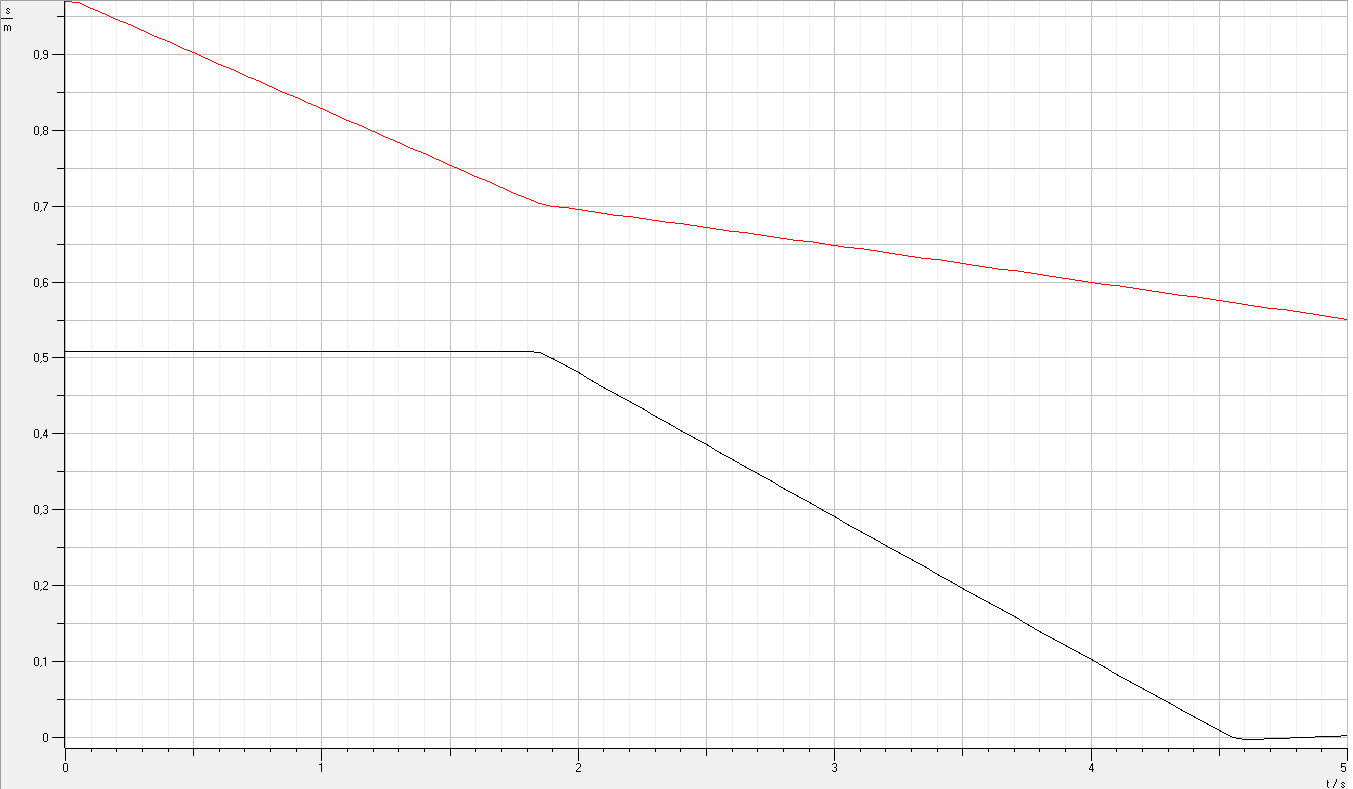
\includegraphics[height=19em]{Data/400-200ela01.png}
\end{figure}

\begin{figure}[h]
    \caption[Graphique vitesse Choc élastique 400g-200g]{Graphique vitesse Choc élastique 400g-200g}
    \centering
    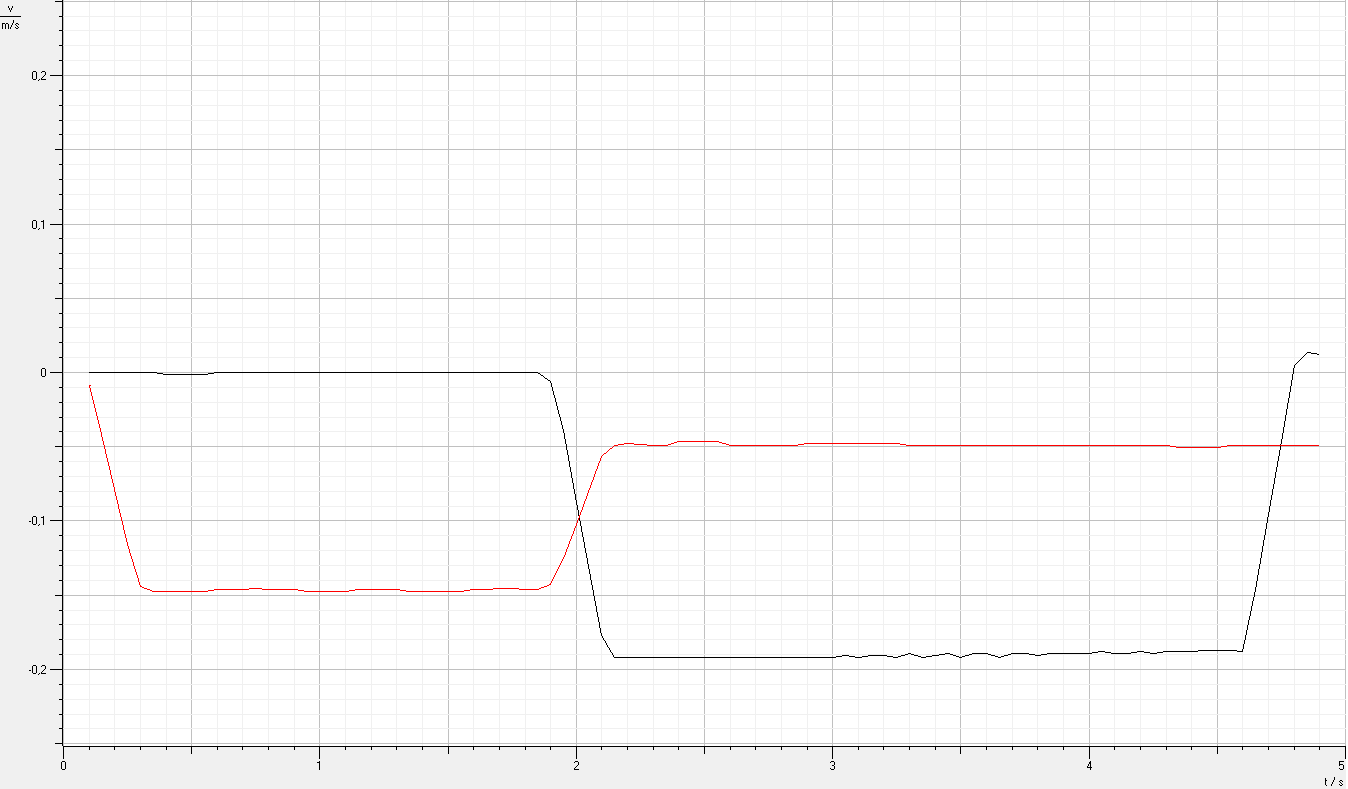
\includegraphics[height=19em]{Data/400-200ela02v.png}
\end{figure}

\newpage

\begin{figure}[h]
    \caption[Graphique accélération Choc élastique 400g-200g]{Graphique accélération Choc élastique 400g-200g}
    \centering
    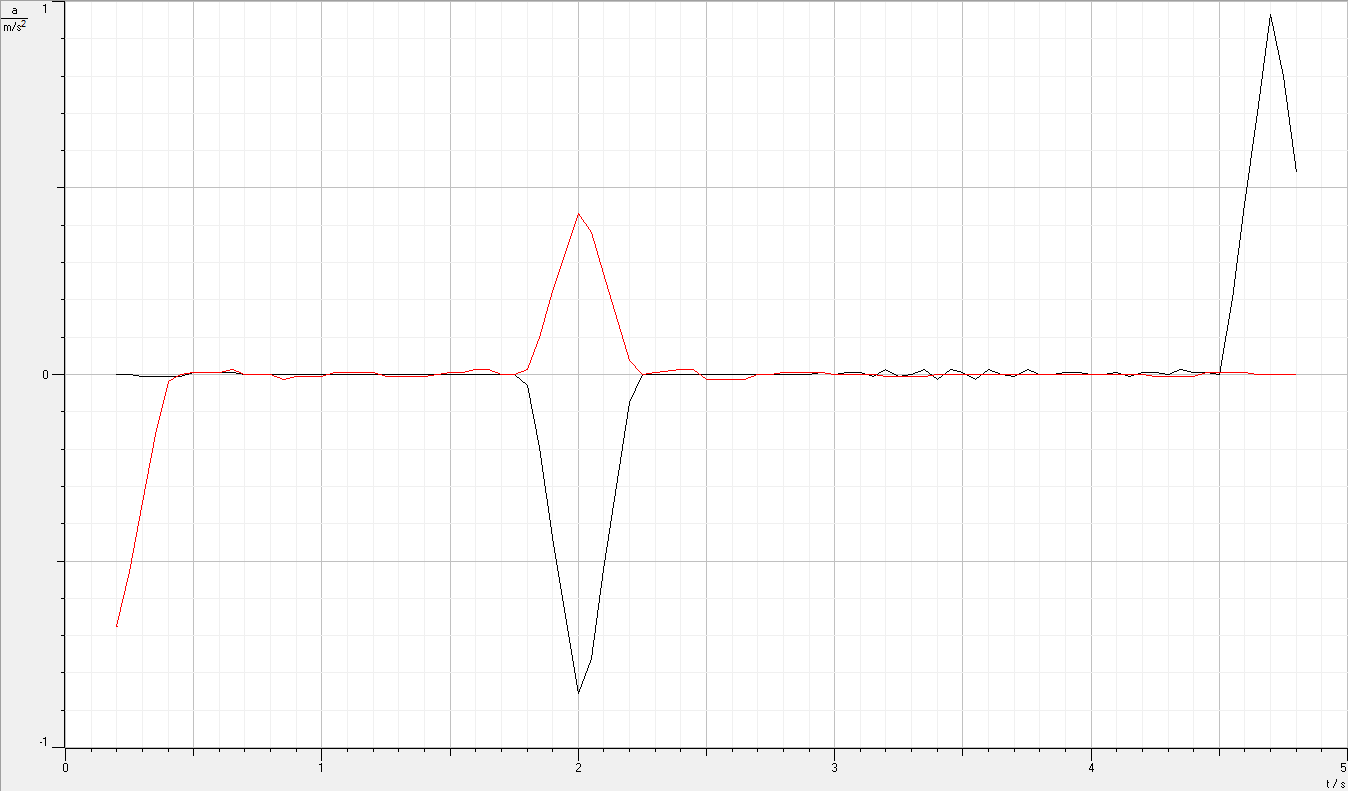
\includegraphics[height=19em]{Data/400-200ela02a.png}
\end{figure}

%%%%%%%%%%%%%%%%%%%%%%%%%%%%%%%%%%%%%%%%%%%%%%%%%%%%%%%%%%%%%%%%%%%%%%%%%%%%%%%%%
\paragraph{Observation préliminaires}
Sur le graphique de position, on voit très clairement le moment du choc et la vitesse à laquelle chacun des chariots continue sa course.
Sur celui de la vitesse c'est un peu plus complexe. Pour le moment il est juste possible d'affirmer que suite aux chocs les deux mobiles restent en mouvement mais pas de manière équivalente.
Sur ce dernier graphique, il est assez explicite que la valeur de l'accélération de chaque chariot est largement différente. Il serait tentant de supposer que l'une vaut la moitié de l'autre. On peut aussi observer la poussée initiale donnée par le lanceur.

\newpage

\begin{figure}[h]
    \caption[Graphique position Choc élastique 200g-200g]{Graphique position Choc inélastique 200g-200g}
    \centering
    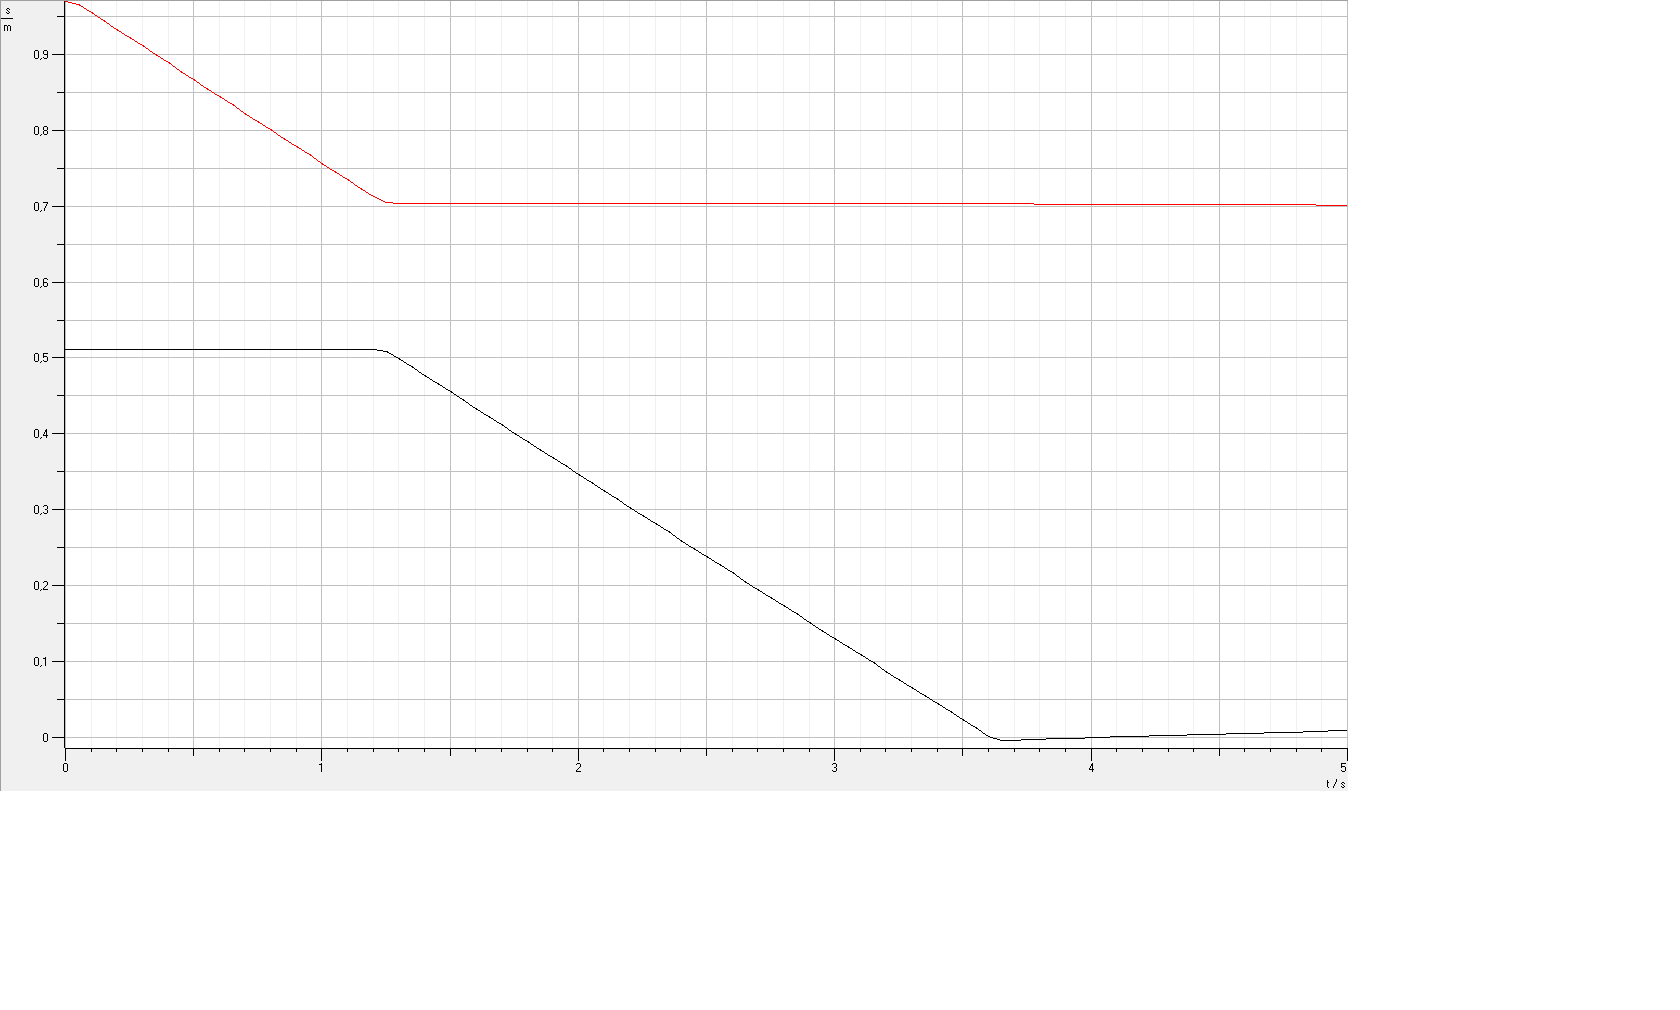
\includegraphics[height=19em]{Data/200-200ela01.png}
\end{figure}

\begin{figure}[h]
    \caption[Graphique vitesse Choc élastique 200g-200g]{Graphique vitesse Choc inélastique 200g-200g}
    \centering
    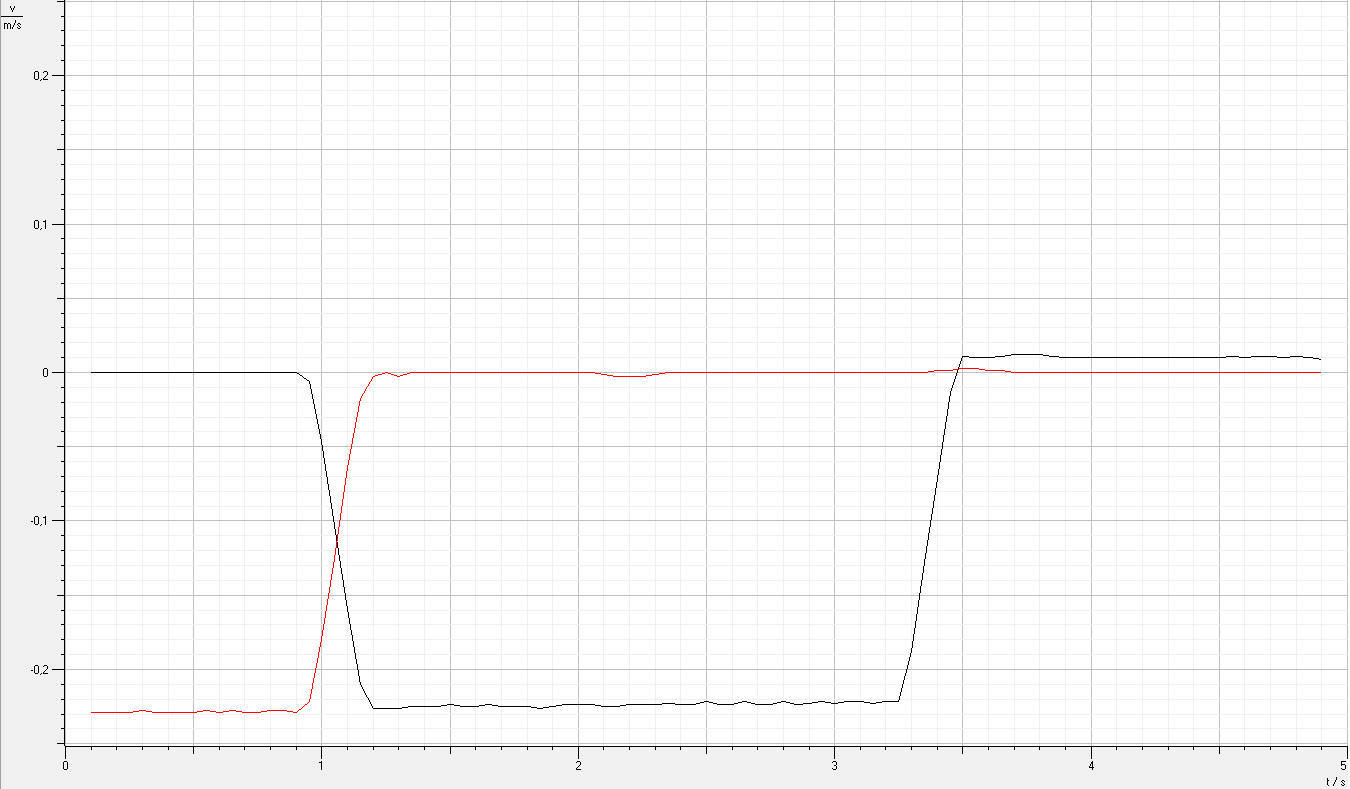
\includegraphics[height=19em]{Data/200-200ela02v.png}
\end{figure}

\newpage

\begin{figure}[h]
    \caption[Graphique accélération Choc élastique 200g-200g]{Graphique accélération Choc inélastique 200g-200g}
    \centering
    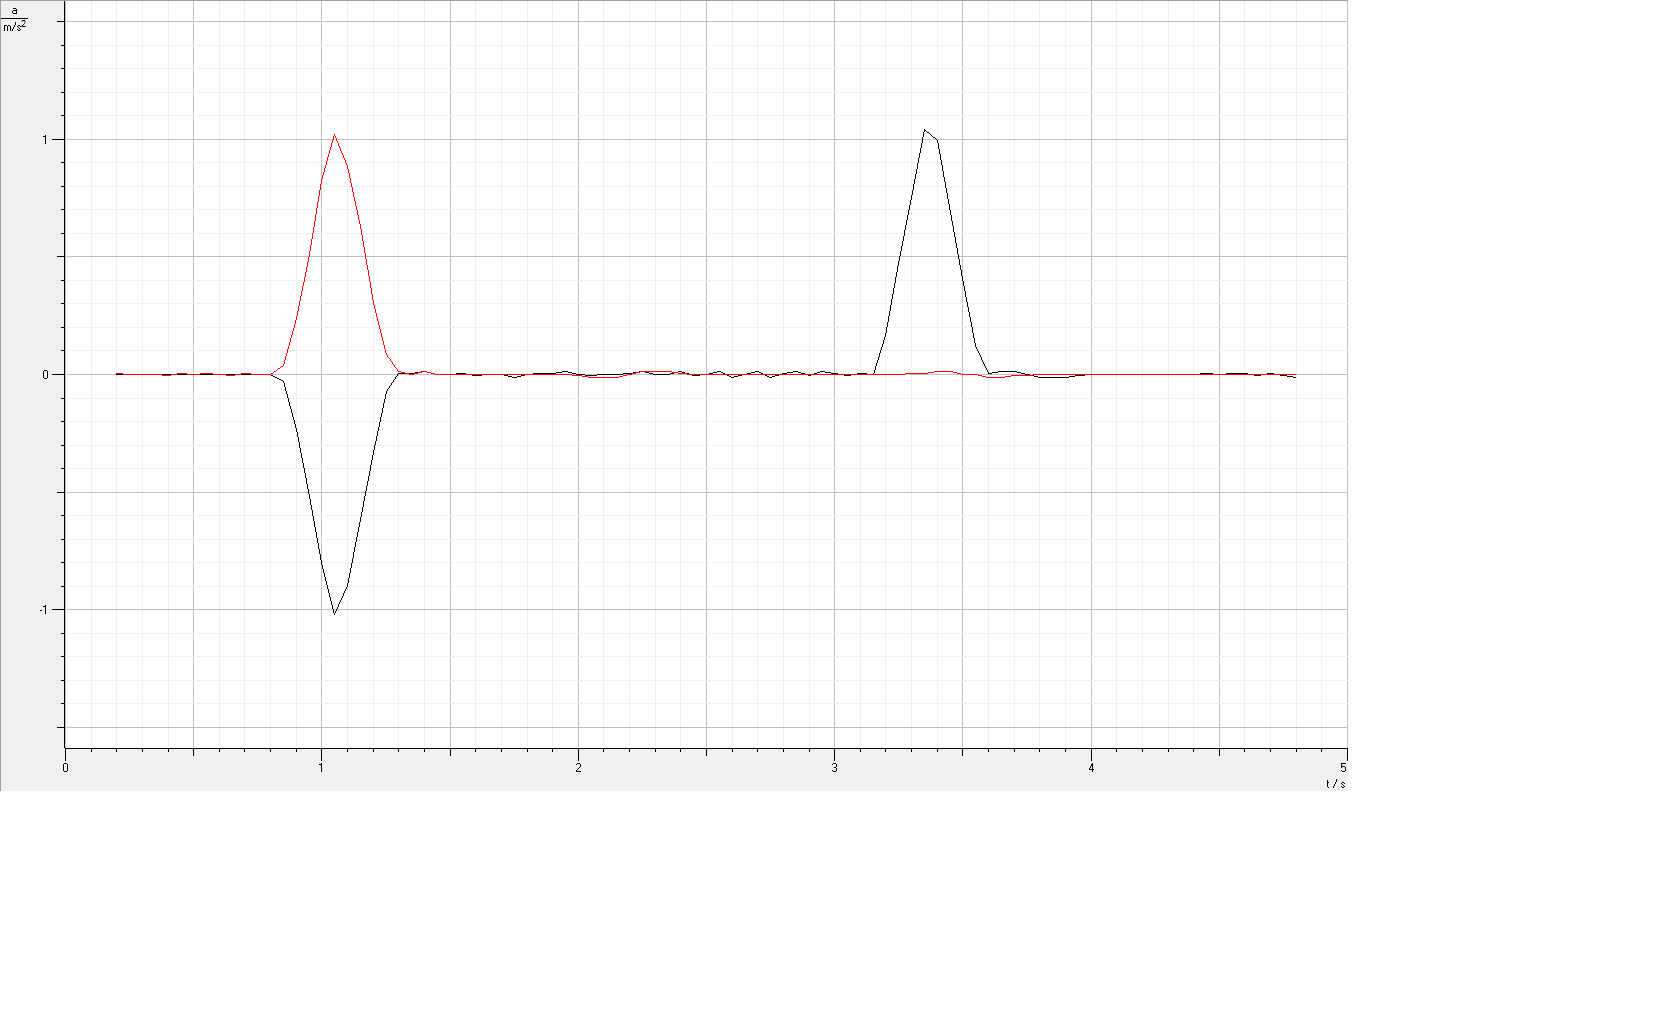
\includegraphics[height=19em]{Data/200-200ela02a.png}
\end{figure}

%%%%%%%%%%%%%%%%%%%%%%%%%%%%%%%%%%%%%%%%%%%%%%%%%%%%%%%%%%%%%%%%%%%%%%%%%%%%%%%%%
\paragraph{Observation préliminaires}

Comme on peut le constater sur les graphiques de vitesse et de position, tout le mouvement d'un chariot est transféré à l'autre au moment du choc. Le premier mobile s'arrêtant alors sur place et le second partant avec la vitesse du premier. L'accéleration est de valeur égale est opposé pour chacun des chariots.

\newpage

\begin{figure}[h]
    \caption[Graphique position Choc inélastique 400g-200g]{Graphique position Choc inélastique 400g-200g}
    \centering
    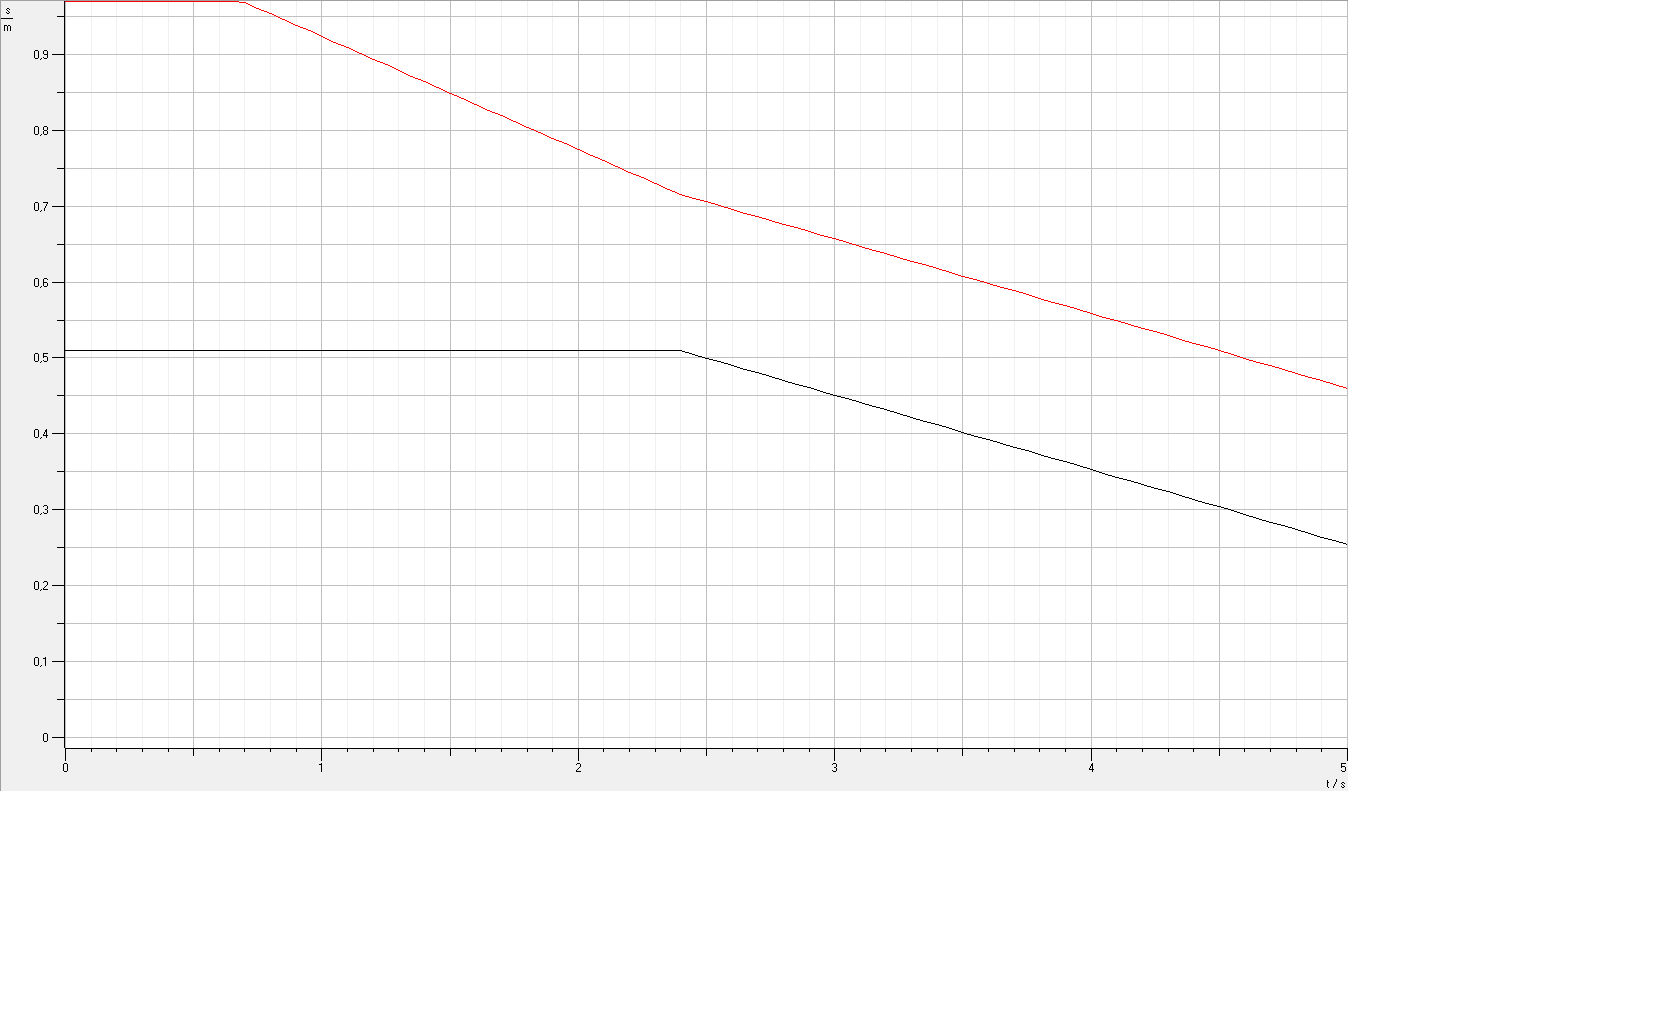
\includegraphics[height=19em]{Data/400-200inela01.png}
\end{figure}

\begin{figure}[h]
    \caption[Graphique vitesse Choc inélastique 400g-200g]{Graphique vitesse Choc inélastique 400g-200g}
    \centering
    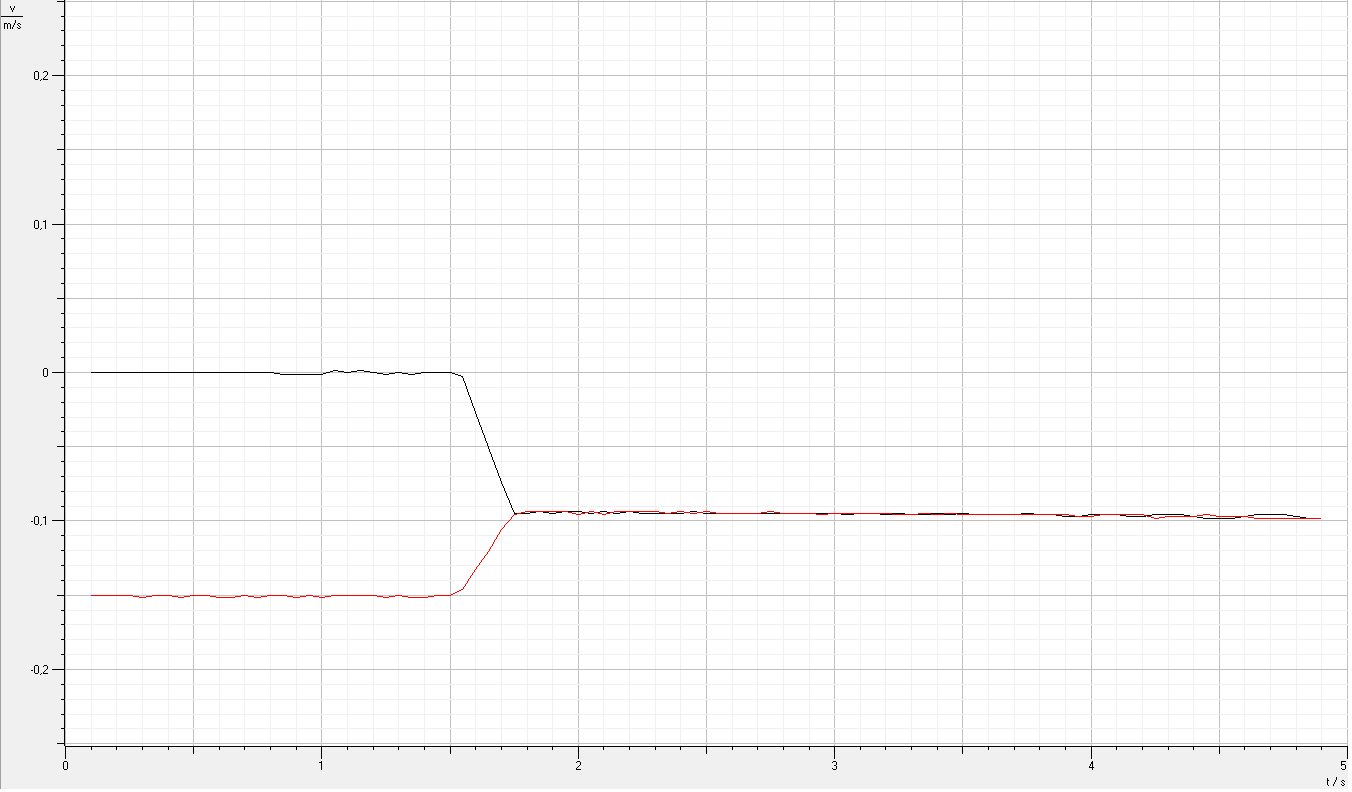
\includegraphics[height=19em]{Data/400-200inela02v.png}
\end{figure}

\newpage

\begin{figure}[h]
    \caption[Graphique accélération Choc inélastique 400g-200g]{Graphique accélération Choc inélastique 400g-200g}
    \centering
    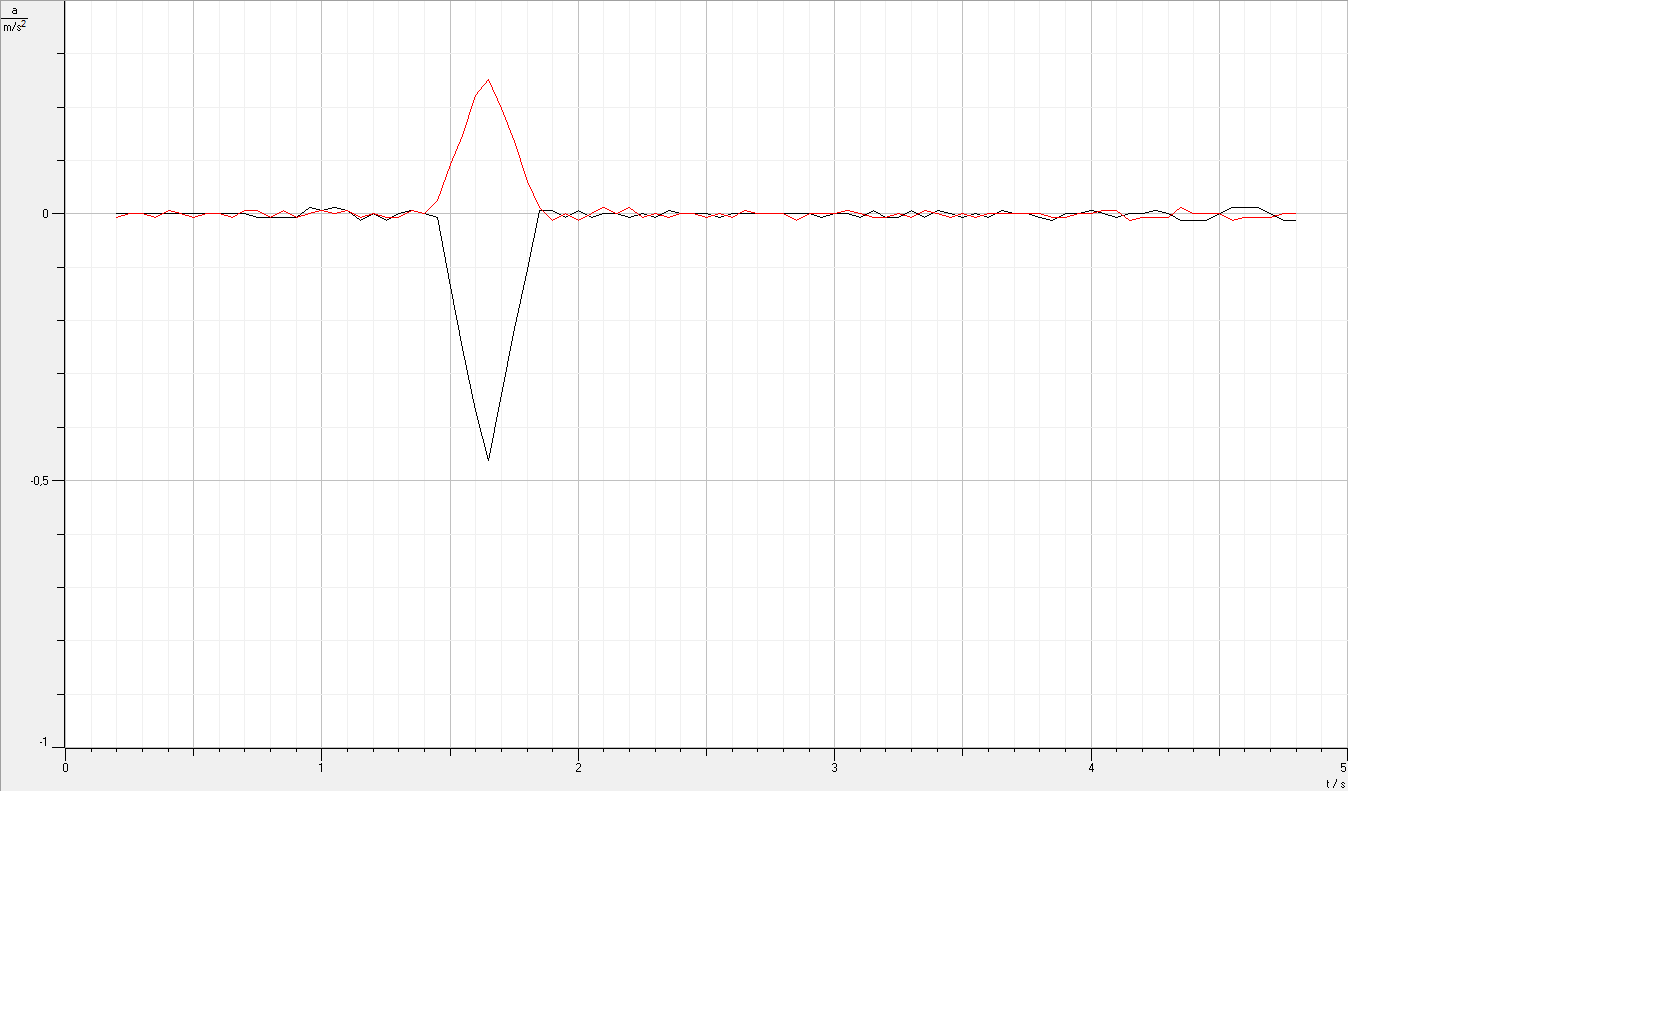
\includegraphics[height=19em]{Data/400-200inela02a.png}
\end{figure}

%%%%%%%%%%%%%%%%%%%%%%%%%%%%%%%%%%%%%%%%%%%%%%%%%%%%%%%%%%%%%%%%%%%%%%%%%%%%%%%%%
\paragraph{Observation préliminaires}

\newpage

\begin{figure}[h]
    \caption[Graphique position Choc inélastique 200g-200g]{Graphique position Choc inélastique 200g-200g}
    \centering
    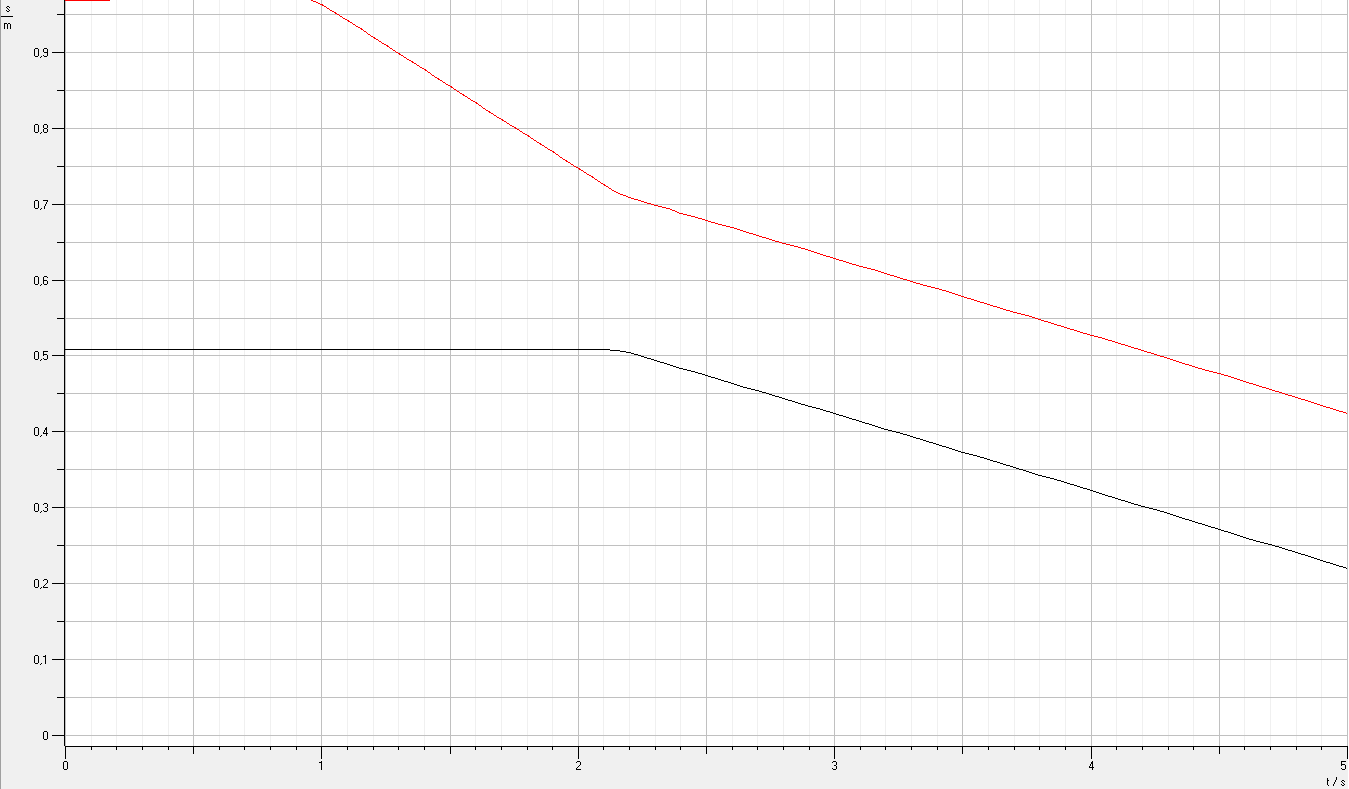
\includegraphics[height=19em]{Data/200-200inela01.png}
\end{figure}

\begin{figure}[h]
    \caption[Graphique vitesse Choc inélastique 200g-200g]{Graphique vitesse Choc inélastique 200g-200g}
    \centering
    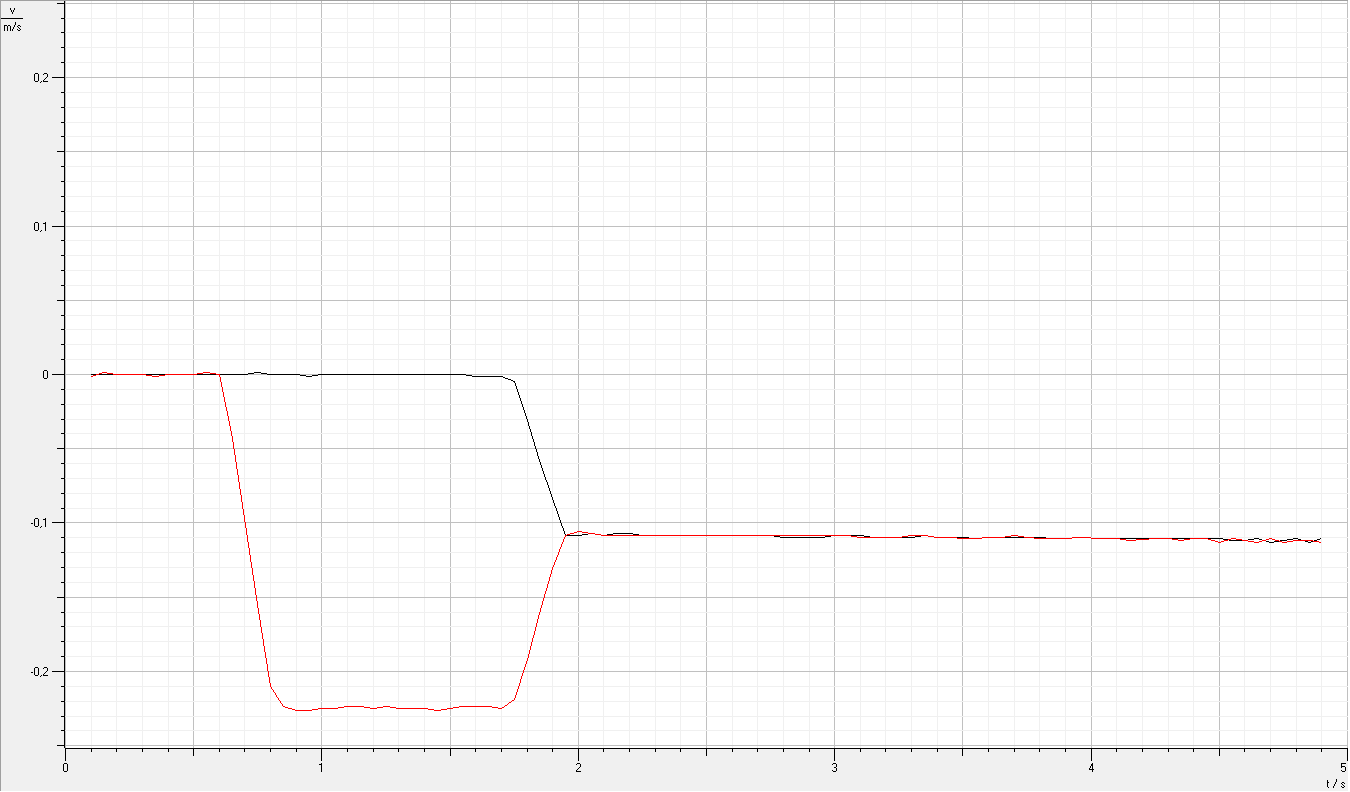
\includegraphics[height=19em]{Data/200-200inela02v.png}
\end{figure}

\newpage

\begin{figure}[h]
    \caption[Graphique accélération Choc inélastique 200g-200g]{Graphique accélération Choc inélastique 200g-200g}
    \centering
    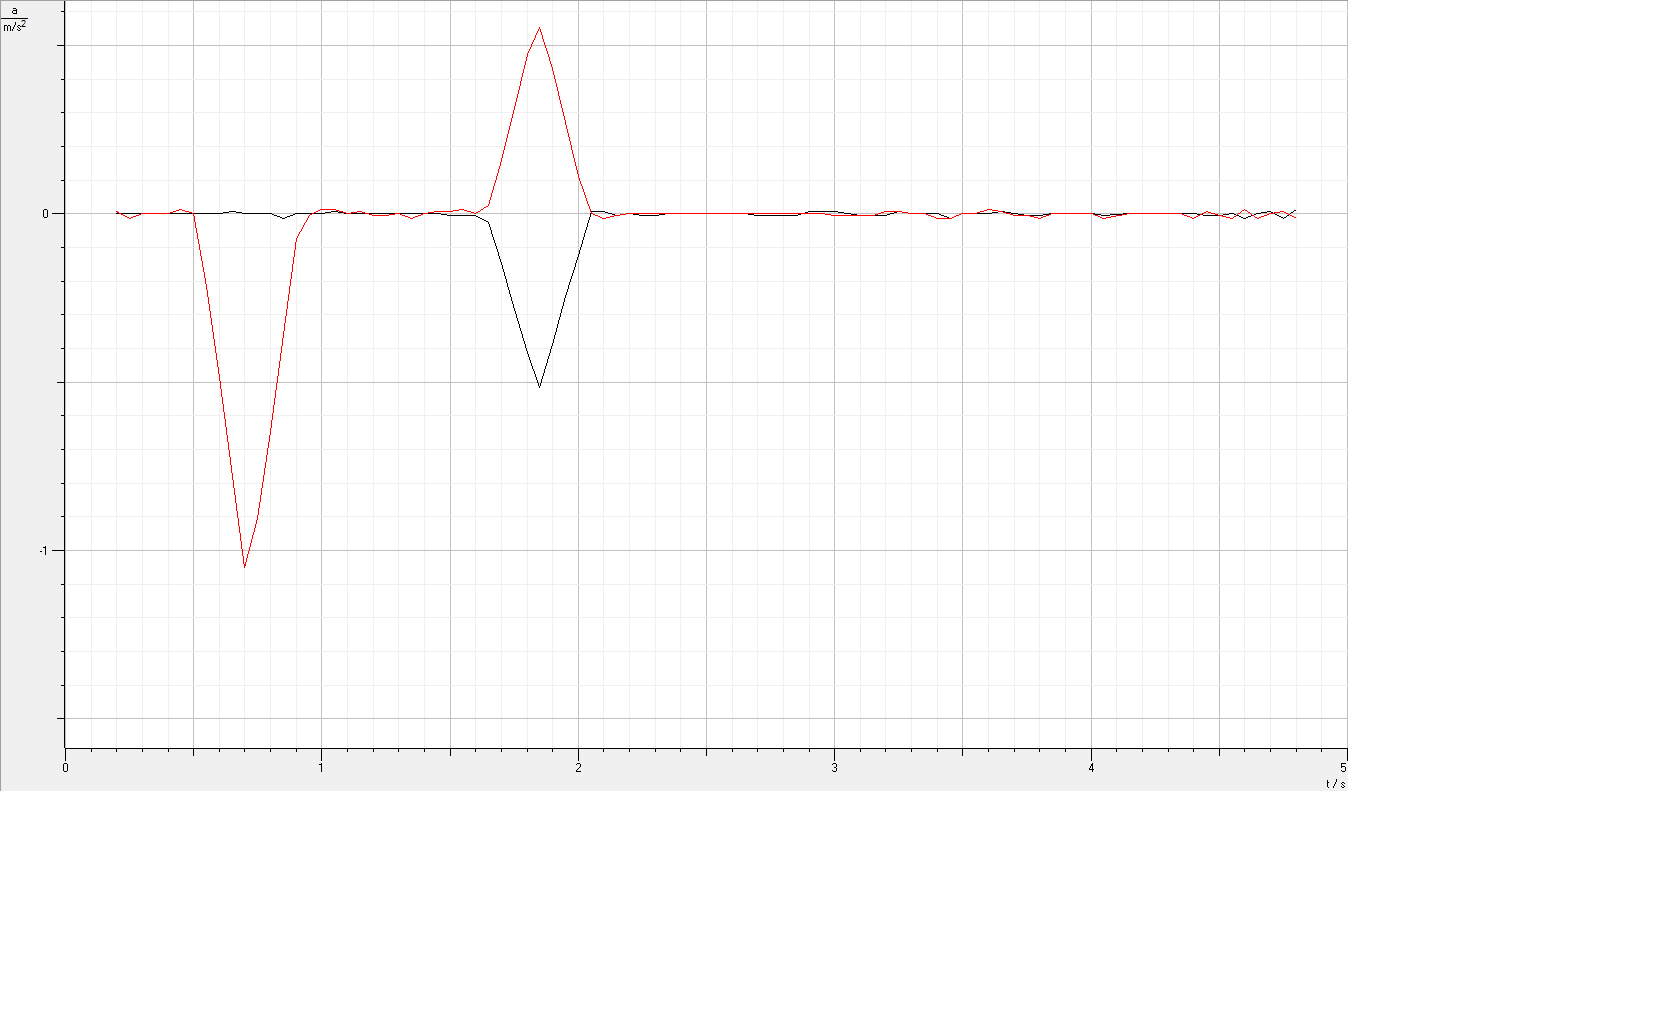
\includegraphics[height=19em]{Data/200-200inela02a.png}
\end{figure}

%%%%%%%%%%%%%%%%%%%%%%%%%%%%%%%%%%%%%%%%%%%%%%%%%%%%%%%%%%%%%%%%%%%%%%%%%%%%%%%%%
\paragraph{Observation préliminaires}
On peut très clairement voir les deux chariots se coller et poursuivre leur trajectoire ensemble.
À la différence du cas élastique, on observe ici 'à l'oeil' que la vitesse finale des deux mobiles réunis est la moyenne de chacun d'entre eux avant la collision.

%%%%%%%%%%%%%%%%%%%%%%%%%%%%%%%%%%%%%%%%%%%%%%%%%%%%%%%%%%%%%%%%%%%%%%%%%%%%%%%%%
\subsection{Conclusion}
En conclusion, la nature quadratique de la loi régissant l'accéleration d'un objet qu'on pourrait assimiler à un point matériel a pu être observée dans des conditions correctes.
La conservation de la quantité de mouvement a, elle aussi pu être constatée. Les incertitudes qui subsistent sont développées dans la conclusion qui suit.
En annexe sont présentes les données supplémentaires que nous avons recueillies lors de l'expérience et les documents nous ayant permis d'achever notre travail.
